%
% Das Poincaré-Lemma
%
\section{Das Poincaré-Lemma
\label{buch:pformen:section:poincarelemma}}
Das Poincaré-Lemma besagt, dass auf einem zusammenziehbaren Gebiet jede
geschlossene $p$-Form exakt ist.
Falls $d\omega=0$ ist, muss es also eine $p-1$-Form $\alpha$ geben mit
$d\alpha=\omega$.
Für geschlossene 1-Formen wurde dies bereits mit Hilfe von Kurvenintegralen
gezeigt.
In diesem Abschnitt soll diese Aussage für beliebige $p$-Formen
nachgewiesen werden.
Zu jeder geschlossenen $p$-Form muss eine Form geringeren Grades gefunden
werden, es müssen also irgendwie einzelne Faktoren $dx^i$ in Funktionen
umgewandelt werden.
Die Faser-Integration, die in
Abschnitt~\ref{buch:pformen:poincare:subsection:faserintegration}
definiert wird, erreicht dies.
Der Fall der 1-Formen verwendete die Wegunabhängigkeit von Wegintegralen
oder die Deformation von Wegen für die Konstruktion der Funktion.
Diese Idee der Deformation wird
in Abschnitt~\ref{buch:pformen:poincare:subsection:homotopie}
mit der Homotopie-Abbildung verallgemeinert.

%
% Homotopie und Restriktion
%
\subsection{Homotopie und Restriktion}
%
% fig-homotopie.tex
%
% (c) 2025 Prof Dr Andreas Müller
%
\begin{figure}
\centering
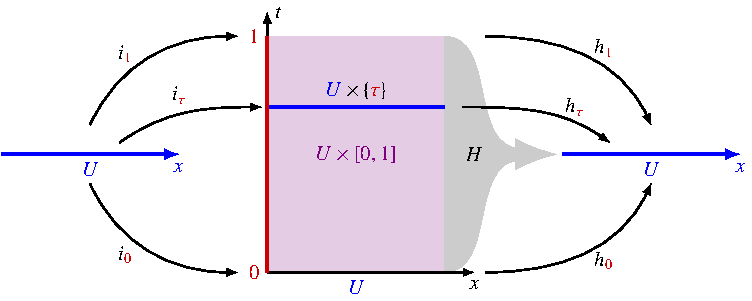
\includegraphics{chapters/060-pformen/images/homotopie.pdf}
\caption{Eine Homotopie $H$ ist eine Abbildung $U\times[0,1]$, die
die Abbildung $h_0\colon U\to U$ in die Abbildung $h_1\colon U\to U$
deformiert.
Die Abbildung $h_{\tau}$ entsteht durch Einsetzen des Wertes $\tau$
in das zweite Argument von $H$, was gleichbedeutend ist mit der
Zusammensetzung von $H$ mit $i_\tau$: $h_\tau=H\circ i_\tau$.
\label{buch:pformen:fig:homotopie}}
\end{figure}
%
Ist die 1-Form $\alpha$ auf einem offenen Ball $U\subset \mathbb{R}^n$
geschlossen, dann kann man eine Funktion $f$ finden, deren Differential
$df=\alpha$ ist.
Die Funktion $f$ entsteht durch Wegintegration z.~B.~vom Nullpunkt zum
Punkt $x$
\[
\gamma_x
\colon [0,1] \to U
:
t\mapsto \gamma_x(t) = xt.
\]
Betrachtet man $\gamma_x(t)$ als eine Funktion von zwei Variablen
$x$ und $t$, dann kann man sie schreiben als
\[
H
\colon
U\times[0,1]
\to
U
:
(x,t) \mapsto tx.
\]
Für jeden Wert von $t$ ist die partielle Funktion
\[
h_t \colon U \to U : x \mapsto tx
\]
eine Selbstabbildung von $U$.
Für $t=0$ wird jeder Punkt auf $0$ abgebildet, die Abbildung $h_0$ ist
die konstante Abbildung auf den Nullpunkt von $U$.
Fpr $t=1$ ist $h_1(x)=x$, $h_1$ ist also die identische Abbildung 
Man nennt $H$ eine {\em Homotopie} zwischen der konstanten Abbildung
und der identischen Abbildung.

Das Definitionsgebiet der Homotopie ist das karteische Produkt
$U\times[0,1]$.
Für jeden Wert von $\tau\in[0,1]$ ist die Abbildung
\[
i_\tau
\colon U \to U\times[0,1]
:
x\mapsto (x,\tau)
\]
eine Einbettung der $n$-dimensionalen Untermannigfaltigkeit $U$ in
$U\times[0,1]$.
Eine $p+1$-Form $\omega$ auf $U\times[0,1]$ wird durch $i_\tau^*$ zu
einer $i_\tau^*(\omega)$, die auf
\begin{align*}
i_\tau^*\bigl(
f(x,t)
\,dx^{i_1}\wedge \dots \wedge dx^{i_p}\wedge dt
\bigr)
&=
0
\\
i_\tau^*\bigl(
g(x,t)
\,dx^{i_1}\wedge \dots \wedge dx^{i_p}\wedge dx^{i_{p+1}}
\bigr)
&=
g(x,\tau)
\,dx^{i_1}\wedge \dots \wedge dx^{i_p}\wedge dx^{i_{p+1}}.
\end{align*}
Die Variable $t$ wird als Konstante mit dem Wert $\tau$ betrachtet.

%
% Faserintegration
%
\subsection{Faserintegration
\label{buch:pformen:poincare:subsection:faserintegration}}
%
% fig-faserintegration.tex
%
% (c) 2025 Prof Dr Andreas Müller
%
\begin{figure}
\centering
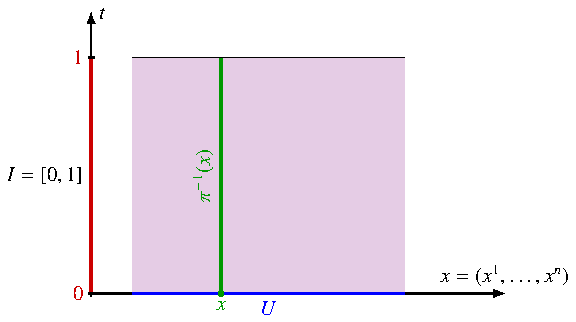
\includegraphics{chapters/060-pformen/images/faserintegration.pdf}
\caption{Die Projektion $\pi(x,t)=x$ projiziert die grünen Fasern
auf Punkte in $U$. Die Faserintegration integriert über solche Fasern
und reduziert damit den Grad einer $p+1$-Form auf $U\times [0,1]$
auf eine $p$-Form.
\label{buch:pformen:poincarelemma:fig:faserintegration}}
\end{figure}
%
Zu jeder $p+1$-Form $\omega$ mit $d\omega=0$ muss eine $p$-Form gefunden
werden.
Dazu müssen einzelne Faktoren $dx^i$ in einem Produkt
$dx^{i_1}\wedge\dots\wedge dx^{i_{p+1}}$ zum Verschwinden gebracht
werden.
Die einzige Möglichkeit, dies zu tun, ist über einzelne Koordinaten zu
integrieren.
Dies ist das Prinzip der Faser-Integration, die im folgenden Satz
definiert wird.

Für den Rest dieses Abschnitts verwenden wir folgende Notation.
Da es nur um lokale Fragen geht, können wir uns auf einzelne
Kartengebiete beschränken.
Wir betrachten daher Differentialformen auf einem offenen Ball
$U\subset\mathbb{R}^n$, in dem wir die Koordinaten mit $x^1,\dots,x^n$
bezeichnen.
Die Projektion $\pi$ ist die Abbildung
\[
\pi
\colon U \times [0,1]\to U : (x,t) \mapsto x,
\]
sie ist in Abbildung~\ref{buch:pformen:poincarelemma:fig:faserintegration}
dargestellt.

Die Projektion $\pi$ ermöglicht, eine $p$-Form $\omega$ auf $U$ in eine
$p$-Form $\pi^*(\omega)$ auf $U\times [0,1]$ abzubilden.
Wir benötigen aber eine andere Art von Abbildung.
Aus einer $p+1$-Form auf $U\times[0,1]$ möchten wir eine $p$-Form auf
$U$ erzeugen.
Dazu integrieren wir über die $t$-Koordinate, wie in der folgenden
Definition.

\begin{definition}
Die {\em Faserintegration} ist die linear Abbildung
\index{Faserintegration}%
$\pi_*\colon \Omega^{p+1}(U\times[0,1])\to\Omega^p(U)$,
die auf Basisformen durch
\begin{align*}
\alpha
&=
a_{i_1 \dots i_p}(x,t)
\,
dx^{i_1}\wedge\dots\wedge dx^{i_p}\wedge dt
&&\Rightarrow&
\pi_*\bigl(
\alpha
\bigr)
&=
\biggl(
\int_0^1 a_{i_1 \dots i_p}(x,t)\,dt
\biggr)
\,
dx^{i_1}\wedge\dots\wedge dx^{i_p}
\\
\beta
&=
b_{i_1 \dots i_{p+1}}(x,t)
\,
dx^{i_1}\wedge \dots \wedge dx^{i_{p+1}}
&&\Rightarrow&
\pi_*\bigl(\beta)
\bigr)
&=
0
\end{align*}
definiert ist.
\end{definition}

Die Faserintegration wirkt also nur auf $p$-Formen, die den Faktor $dt$
enthält.
Solche Faktoren werden über die Variable $t$ integriert.

Die Faserintegration ist nicht aus einer Abbildung der unterliegenden
Mannigfaltigkeiten entstanden (das wäre die Abbildung $\pi^*$).
Daher muss im nächsten Schritt ermittelt werden, wie Faserintegration
sich mit der äusseren Ableitung von Formen verträgt.

\begin{satz}[Faserintegration]
Sei $\omega\in\Omega^{p+1}(U\times[0,1])$ eine $p+1$-Form auf $U\times[0,1]$.
Dann  ist
\begin{equation}
\pi_*d\omega - d\pi_*\omega 
=
(-1)^{p+1}(i_1^*\omega- i_0^*\omega).
\label{buch:pformen:poincarelemma:eqn:pid}
\end{equation}
\end{satz}

\begin{proof}
Wir berechnen die Ableitungen und die Faserintegration der
Basis-$p+1$-Formen
\begin{align*}
\alpha
&=
a_{i_1 \dots i_p}(x,t)
\,
dx^{i_1}\wedge \dots \wedge dx^{i_p}\wedge dt
\\
\beta
&=
b_{i_1 \dots i_p i_{p+1}}(x,t)
\,
dx^{i_1}\wedge \dots \wedge dx^{i_p}\wedge dx^{i_{p+1}}
\end{align*}
auf $U\times[0,1]$.

Da $\alpha$ bereits $dt$ enthält, kommen in $d\alpha$ keine Ableitungen
von $a_{i_1\dots i_p}$ nach der Zeit vorkommen.
Die Ableitungen sind:
\begin{align*}
d\alpha
&=
\sum_{k=1}^n \frac{\partial a_{i_1\dots i_p}(x,t)}{\partial x^k}
\,dx^k\wedge dx^{i_1}\wedge \dots \wedge dx^{i_p}\wedge dt
\\
d\beta
&=
\sum_{k=1}^n \frac{\partial b_{i_1\dots i_{p+1}}(x,t)}{\partial x^k}
\,dx^k\wedge dx^{i_1}\wedge \dots \wedge dx^{i_{p+1}}
+
\frac{\partial b_{i_1\dots i_{p+1}}(x,t)}{\partial t}
\,dt\wedge dx^{i_1}\wedge \dots\wedge dx^{i_{p+1}}
\intertext{Die Faserintegration erhält nur die Terme mit $dt$ und 
ergibt}
\pi_*d\alpha
&=
\sum_{k=1}^n
\biggl(
\int_0^1 \frac{\partial a_{i_1\dots i_p}(x,t)}{\partial x^k}
\,dt
\biggr)
\,
dx^k
\wedge
dx^{i_1}\wedge\dots\wedge dx^{i_p}
\\
\pi_*d\beta
&=
\biggl(
\int_0^1
\frac{\partial b_{i_1 \dots i_{p+1}}(x,t)}{\partial t}
\,dt
\biggr)
\,
(-1)^{p+1}
\,
dx^{i_1}\wedge\dots \wedge dx^{i_{p+1}}
\\
&=
\Bigl(
b_{i_1\dots i_{p+1}}(x,1)
-
b_{i_1\dots i_{p+1}}(x,0)
\Bigr)
\,
(-1)^{p+1}
\,
dx^{i_1}\wedge\dots\wedge dx^{i_p}\wedge dx^{i_{p+1}}
\intertext{Die beiden Summanden im letzten Ausdruck entstehen dadurch,
dass die Variable $t$ auf $0$ bzw.~$1$, das ist}
&=
(-1)^{p+1}
\bigl(
i_1^*\beta - i_0^*\beta
\bigr).
\end{align*}

Wir berechnen jetzt die Wirkung der Operatoren $\pi^*$ und $d$ in der
umgekehrten Reihenfolge.
Da $\pi^*\beta=0$ ist auch $d\pi^*\beta=0$.
Für $\alpha$ ist etwa mehr Arbeit notwendig.
\begin{align*}
d\pi_*\alpha
&=
\sum_{k=1}^n
\frac{\partial}{\partial x_k}
\biggl(
\int_0^1 a_{i_1\dots i_p}(x,t)\,dt
\biggr)
dx^k\wedge dx^{i_1}\wedge\dots\wedge dx^{i_p}
\intertext{Die Ableitung kann ins Integral genommen werden und ergibt}
&=
\sum_{k=1}^n
\biggl(
\int_0^1 \frac{\partial a_{i_1\dots i_p}(x,t)}{\partial x_i} \,dt
\biggl)
\,
dx^k
\wedge
dx^{i_1}\wedge\dots\wedge dx^{i_p}
\\
&=
\pi_*d\alpha.
\end{align*}

Die Rechnung in den vorangegangenen Absätzen zeigt also, dass
\begin{align}
\pi_*d\alpha - d\pi_*\alpha
&=
0,
\label{buch:pformen:poincarelemma:eqn:i*alpha}
\\
\pi_*d\beta - d\pi_*\beta
&=
(-1)^{p+1}
\bigl(
i_1^*\beta - i_0^*\beta
\bigr).
\notag
\end{align}
Da in den Termen der Form $\alpha$ immer der Faktor $dt$ vorkommt, 
der von $i_\tau^*$ auf $0$ abgebildet wird, gilt $i_t^*\alpha=0$
und man kann die Null auf der rechten Seite von 
\eqref{buch:pformen:poincarelemma:eqn:i*alpha}
ebenfalls als
\(
\pi_*d\alpha-d\pi*\alpha=(-1)^{p+1}\bigl(i_1^*\alpha-i_0^*\alpha\bigr)
\)
schreiben.
Damit ist die Formel
\eqref{buch:pformen:poincarelemma:eqn:pid}
bewiesen.
\end{proof}

%
% Homotopie-Abbildung
%
\subsection{Homotopie-Abbildung
\label{buch:pformen:poincare:subsection:homotopie}}
Die Homotopie $H\colon U\times[0,1]\to U$ ist eine differenzierbare
Abbildung.
Die induzierte Abbildung $H^*\colon\Omega^*(U)\to\Omega^*(U\times[0,1])$
vertauscht mit $d$.
Für eine $p$-Form $\omega$ auf $U$ ist $H^*\omega$ eine $p$-Form auf
$U\times[0,1]$.
Entsprechend ist $\pi_*H^*\omega$ ist eine $p-1$-Form auf $U$.
Wir definieren daher die Funktion $J=\pi_*H^*$ und berechnen das
Verhalten mit der äusseren Ableitung.

\begin{satz}
\label{buch:pformen:poincarelemma:satz:homotopie}
Für jede $p$-Form $\omega\in\Omega^p(U)$ gilt
\[
Jd\omega - dJ\omega
=
(-1)^p(
h_1^*\omega - h_0^*\omega
)
\]
\end{satz}

\begin{proof}
\begin{align*}
J d \omega - d J \omega
&=
\pi_* H^* d \omega
-
d \pi^* H^* \omega
\\
&=
\pi_* d H^* \omega
-
d \pi^* H^* \omega
\\
&=
d \pi_* H^* \omega
+
(-1)^p(i_1^* H^* \omega - i_0^* H^* \omega)
-
d \pi^* H^* \omega.
\intertext{Der erste und der letzte Term heben sich weg.
Im mittleren Term ist $H\circ i_\tau=h_\tau$ und daher
$i_\tau^* H^* = (H\circ i_\tau)^* = h_\tau^*$.
Somit folgt}
J d \omega - d J \omega
&=
(-1)^p(h_1^* \omega - h_0^* \omega).
\end{align*}
wie behauptet.
\end{proof}

%
% Geschlossene Formen sind exakt
%
\subsection{Geschlossene Formen sind exakt
\label{buch:pformen:geschlossen:subsection:exakt}}
Mit der Faserintegration und der Homotopie-Abbildung wurde
in Abschnitt~\ref{buch:pformen:poincare:subsection:homotopie}
die Abbildung $J$ konstruiert, deren Eigenschaften im
Satz~\ref{buch:pformen:poincarelemma:satz:homotopie}
zusammengestellt wurden.
Damit ist es jetzt möglich, das Poincaré-Lemma zu beweisen.

\begin{satz}[Poincaré-Lemma]
\label{buch:pformen:geschlossen:satz:poincare-lemma}
Ist die $p$-Form $\omega\in\Omega^p(U)$ geschlossen, also $d\omega=0$,
dann gibt es eine $p-1$-Form $\alpha\in\Omega^{p-1}(U)$ mit
$d\alpha=\omega$.
\end{satz}

\begin{proof}
Nach Satz~\ref{buch:pformen:poincarelemma:satz:homotopie} folgt
wegen $d\omega=0$ sofort
\[
-dJ\omega
=
(-1)^p(h_1^*\omega - h_0^*\omega).
\]
Die Abbildung $h_0$ ist die konstante Abbildung $x\mapsto 0$, also ist ist
$h_0^*\omega=0$.
$h_1$ ist die identische Abbildung $x\mapsto x$, daher ist auch $h_1^*$
die identische Abbildung von $\Omega^*(U)$ und daher $h_1^*\omega=\omega$.
Damit folgt $dJ\omega=\omega$.
Somit ist $\alpha =(-1)^{p+1}J\omega$ die gesuchte $p-1$-Form.
\end{proof}

Wir prüfen nach, dass der ursprünglich für geschlossene 1-Formen
$\omega$ gegebene Beweis die gleiche Funktion
$f=J\omega\in\Omega^0(U)=\mathscr{E}(U)$ mit $df=\omega$ ergibt.
Für eine 1-Form
\[
\omega = \sum_{i=1}^nf_i(x)\, dx^i
\]
Zunächst ist
\[
H^*\omega
=
\sum_{i=1}^nf_i(tx)\, d(tx^i)
=
\sum_{i=1}^nf_i(tx) (x_i\, dt + t\, dx^i).
\]
Darauf muss jetz die Operation $\pi_*$ angewendet werden.
Diese ergibt aber nichtverschwindende Resultat nur auf Termen, in
denen $dt$ vorkommt.
Daher ist
\[
\pi_*H^*\omega
=
\int_0^1
\sum_{i=1}^n
f_i(tx) x^i\, dt
=
\int_0^1
\sum_{i=1}^n
f_i(\gamma_x(t)) \dot{x}^i(t)\, dt
=
\int_{\gamma_x}
\omega.
\]
Die von der Abbildung $J$ produzierte Funktion ist also im Falle
einer 1-Form gerade das Wegintegral über einen Weg vom Nullpunkt zum
Punkt $x$, wie in der ursprünglichen Konstruktion in
Kapitel~\ref{chapter:kurvenintegral}.



